% !TEX program = xelatex
% =============================================================================
%  全国大学生数学建模竞赛（CUMCM）LaTeX 模板
%  对应 Typst 模板 zh/cumcm/main.typ 的全部功能。
%
%  字体依赖（正文宋体 / 标题黑体 / 强调楷体）：
%    - 规范字体：SimSun（宋体）、SimHei（黑体）、KaiTi（楷体）。
%    - 本模板默认使用 ctex 的 fontset=mac，在 macOS 上自动选用同族等价字体
%      Songti SC / Heiti SC / Kaiti SC，确保开箱即用。
%    - 若系统已安装 SimSun/SimHei/KaiTi（如 Windows 或手动安装），可将下方
%      \documentclass 选项 fontset=mac 改为 fontset=windows，即可使用规范字体。
%    - 西文正文：Times New Roman；代码等宽：Menlo（缺失时回退到默认字体）。
%  编译方式：xelatex main.tex （需运行两遍以生成目录）
% =============================================================================
\documentclass[fontset=fandol, 12pt, a4paper]{ctexart}

% ---------- 页面：A4，上下左右 2.5cm ----------
\usepackage[a4paper, top=2.5cm, bottom=2.5cm, left=2.5cm, right=2.5cm]{geometry}

% ---------- 数学 ----------
\usepackage{amsmath,amssymb}

% ---------- 图片、浮动体与交叉引用 ----------
\usepackage{graphicx}
\usepackage{float}
\usepackage{caption}
\usepackage[hidelinks]{hyperref}

% ---------- 字体（fontspec + ctex，xelatex 编译） ----------
% 中文宋体/黑体/楷体由 ctex 的 fontset=fandol 自动设置，
% 并自动定义 \songti / \heiti / \kaishu 等字体命令。

% ---------- 正文：12.05pt，首行缩进 2em，两端对齐，行距 0.72em ----------
% 12pt 字号近似 12.05pt；0.72em 行距 => 行高 = 1.72 * 字号，\linespread 因子 ≈ 1.43
\linespread{1.43}
\setlength{\parindent}{2em}

% ---------- 标题编号（\ctexset 配置） ----------
% 一级标题用中文数字“一、二、三、”，二级及以下用 1.1 / 1.1.1
\ctexset{
  section/number       = \chinese{section},
  subsection/number    = \arabic{section}.\arabic{subsection},
  subsubsection/number = \arabic{section}.\arabic{subsection}.\arabic{subsubsection},
}

% ---------- 标题格式（titlesec 配置） ----------
\usepackage{titlesec}
\titleformat{\section}
  {\centering\fontsize{17.3pt}{20.8pt}\heiti\bfseries}
  {\chinese{section}、}{1em}{}
\titleformat{\subsection}
  {\fontsize{14.45pt}{17.4pt}\heiti\bfseries}
  {\arabic{section}.\arabic{subsection}}{1em}{}
\titleformat{\subsubsection}
  {\fontsize{12.05pt}{14.5pt}\heiti\bfseries}
  {\arabic{section}.\arabic{subsection}.\arabic{subsubsection}}{1em}{}
\titlespacing{\section}       {0pt}{1.25em}{0.82em}
\titlespacing{\subsection}    {0pt}{1.15em}{0.55em}
\titlespacing{\subsubsection} {0pt}{1.15em}{0.55em}

% ---------- 目录（tocloft 点线引导） ----------
\usepackage{tocloft}
\renewcommand{\cftsecfont}{\heiti\bfseries}
\renewcommand{\cftsecpagefont}{\heiti\bfseries}
\renewcommand{\cftsecleader}{\cftdotfill{\cftdotsep}}
\renewcommand{\cftsubsecleader}{\cftdotfill{\cftdotsep}}
\renewcommand{\cftsubsubsecleader}{\cftdotfill{\cftdotsep}}

% ---------- 表格与代码 ----------
\usepackage{booktabs}
\usepackage{array}
\usepackage{xcolor}
\usepackage{listings}
\lstset{
  basicstyle=\ttfamily\small,
  backgroundcolor=\color{black!3},
  frame=single,
  framesep=6pt,
  rulecolor=\color{black!30},
  framerule=0.8pt,
  breaklines=true,
  showstringspaces=false,
  columns=fullflexible,
  keepspaces=true,
}

% ---------- 页码：底部居中 ----------
\pagestyle{plain}

% ---------- 自定义命令（对应 Typst 函数） ----------
% \papertitle{标题}：居中 17.3pt 加粗标题
\newcommand{\papertitle}[1]{%
  \thispagestyle{empty}%
  \begin{center}
    {\fontsize{17.3pt}{22pt}\bfseries #1}
  \end{center}
  \vspace{1em}
}
% \abstractcn{摘要正文}{关键词}：居中“摘要”标题（14pt 加粗）+ 正文 + “关键字：”加粗 + 关键词 + 换页
\newcommand{\abstractcn}[2]{%
  \thispagestyle{empty}%
  \begin{center}{\fontsize{14pt}{17pt}\bfseries 摘要}\end{center}
  #1\par
  \vspace{1em}
  {\heiti\bfseries 关键字：}#2\par
  \newpage
}
% \tocpage：目录页，标题“目录”居中 17.3pt 黑体加粗，点线引导
\makeatletter
\newcommand{\tocpage}{%
  \setcounter{page}{1}%
  \begin{center}
    {\fontsize{17.3pt}{20.8pt}\heiti\bfseries 目录}
  \end{center}
  \vspace{0.5em}
  \@starttoc{toc}%
  \newpage
}
\makeatother
% \referencescn：参考文献节，标题“参考文献”（不带编号但进目录）
\newcommand{\referencescn}{%
  \addcontentsline{toc}{section}{参考文献}%
  % 参考文献。注意：main.tex 中 \referencescn 已通过 thebibliography 自动生成
% “参考文献”一级标题（不带编号），并已 \addcontentsline 进入目录，
% 所以本文件**不要再写一级标题**，否则会出现两个“参考文献”标题。

\begin{thebibliography}{99}
\bibitem{ref1} Lo Y M D, Corbetta N, Chamberlain P F, et al. Presence of fetal DNA in maternal plasma and serum[J]. The Lancet, 1997, 350(9076): 485--487.
\bibitem{ref2} Ashoor G, Syngelaki A, Poon L C Y, et al. Fetal fraction in maternal plasma cell-free DNA at 11--13 weeks' gestation: relation to maternal and fetal characteristics[J]. Ultrasound in Obstetrics \& Gynecology, 2013, 41(1): 26--32.
\bibitem{ref3} Norton M E, Jacobsson B, Swamy G K, et al. Cell-free DNA analysis for noninvasive examination of trisomy[J]. New England Journal of Medicine, 2015, 372(17): 1589--1597.
\bibitem{ref4} Wang E, Batey A, Struble C, et al. Gestational age and maternal weight effects on fetal cell-free DNA in maternal plasma[J]. Prenatal Diagnosis, 2013, 33(7): 662--666.
\bibitem{ref5} Bianchi D W, Chiu R W K. Sequencing of circulating cell-free DNA during pregnancy[J]. New England Journal of Medicine, 2018, 379(5): 464--473.
\bibitem{ref6} 李金明. 无创产前检测技术的临床应用与质量控制[J]. 中华检验医学杂志, 2016, 39(5): 321--324.
\end{thebibliography}
%
}
% \appendixcn：附录节，标题“附录 A  核心代码”
\newcommand{\appendixcn}{%
  \section*{附录 A\quad 核心代码}%
  \addcontentsline{toc}{section}{附录 A\quad 核心代码}%
  % 附录：核心代码（关键片段，完整代码见 code/ 目录）

\textbf{1. 孕周解析与达标指标（utils.py 核心）}

\begin{lstlisting}[language=Python]
def parse_wk(s):
    t = str(s).lower()
    if "w" not in t:
        return float("nan")
    w = float(t.split("w")[0])
    d = float(t.split("+")[1]) if "+" in t else 0.0
    return w + d / 7.0

THETA = 0.04  # Y 染色体浓度达标阈值
male["孕周"] = male["检测孕周"].apply(parse_wk)
male["达标"] = (male["Y染色体浓度"] >= THETA).astype(int)
\end{lstlisting}

\textbf{2. 问题一面板分解与混合效应模型}

\begin{lstlisting}[language=Python]
import statsmodels.formula.api as smf
# 组内去均值（固定效应）
df["y_w"] = df["y"] - df.groupby("code")["y"].transform("mean")
df["week_w"] = df["week"] - df.groupby("code")["week"].transform("mean")
fe = smf.ols("y_w ~ week_w - 1", data=df).fit()   # 组内孕周斜率
# 组间 BMI
gb = df.drop_duplicates("code")
between = smf.ols("y_mean ~ bmi_mean", data=gb).fit()  # 组间 BMI 效应
# 混合效应模型
me = smf.mixedlm("y ~ week + bmi", data=df, groups=df["code"]).fit(reml=True)
\end{lstlisting}

\textbf{3. 问题二达标时间估计与最佳时点}

\begin{lstlisting}[language=Python]
BETA1 = 0.00319  # 问题一固定效应斜率
df["adj"] = df["y"] - BETA1 * df["week"]
person = df.groupby("code").agg(a=("adj", "mean"), bmi=("bmi", "mean")).reset_index()
person["tstar"] = (THETA - person["a"]) / BETA1   # 个体达标时间
# BMI 分组，取组内 90% 分位作为最佳时点
person["group"] = pd.cut(person["bmi"], bins=[20,28,32,36,40,60], right=False)
best = person.groupby("group")["tstar"].quantile(0.9)
\end{lstlisting}

\textbf{4. 问题四女胎异常判定（随机森林 + 交叉验证）}

\begin{lstlisting}[language=Python]
from sklearn.ensemble import RandomForestClassifier
from sklearn.model_selection import StratifiedKFold, cross_val_predict
skf = StratifiedKFold(n_splits=5, shuffle=True, random_state=42)
rf = RandomForestClassifier(n_estimators=500, class_weight="balanced", random_state=42)
rf_prob = cross_val_predict(rf, X, y, cv=skf, method="predict_proba")[:, 1]
auc = roc_auc_score(y, rf_prob)   # AUC = 0.789
\end{lstlisting}
%
}
% \threelinetable{标题}{列定义}{表头}{表格内容}：三线表，标题在表格上方居中 10.5pt 黑体加粗
% 调用示例：\threelinetable{表 1 示例}{ccc}{A & B & C}{1 & 2 & 3 \\ 4 & 5 & 6}
\newcommand{\threelinetable}[4]{%
  \begin{center}
    {\fontsize{10.5pt}{12.6pt}\heiti\bfseries #1}\par
    \vspace{0.6em}
    \begin{tabular}{#2}
      \toprule
      #3 \\
      \midrule
      #4 \\
      \bottomrule
    \end{tabular}
  \end{center}
}

\begin{document}

% 封面（不编号）
\papertitle{基于面板数据建模的 NIPT 时点选择与胎儿异常判定}

% 摘要页（不编号）
\abstractcn{%
针对无创产前检测（NIPT）的时点选择与胎儿异常判定问题，本文建立了统计建模与分类判定相结合的一整套方法。

\textbf{针对问题一}，考虑到数据为纵向面板结构，横截面相关存在混杂，本文采用组内/组间分解与混合效应模型分离孕周与 BMI 的效应。结果表明：同一孕妇内 Y 染色体浓度随孕周显著线性上升（固定效应斜率 $0.00319$/周，$t=24.26$，$p<10^{-100}$），孕妇间 BMI 表现为显著负效应（$-0.00222$/BMI，$p<10^{-4}$）；混合效应模型给出关系式 $Y=0.070+0.00313t-0.00138B$，孕周与 BMI 效应均高度显著。

\textbf{针对问题二}，以固定效应斜率估计个体达标时间，回归得到达标时间与 BMI 的关系 $t=-19.46+0.757B$（$p<0.001$）。按 BMI 分组并取组内 90\% 可靠达标的最早时点作为最佳时点：BMI $[28,32)$ 组约 15.5 周、$[32,36)$ 组约 16.1 周、$[36,40)$ 组约 20.1 周，BMI 越高最佳时点越晚。检测误差每增加约 0.005，最佳时点后移约 2 周。

\textbf{针对问题三}，引入身高、体重、年龄多维因素，随机森林显示体重与 BMI 为主导因素；多维 K-means 聚类分组后，高 BMI 组（BMI$\approx36.4$）最佳时点约 20.2 周、低 BMI 组约 14.5 周，且组内同质性优于仅按 BMI 分组。

\textbf{针对问题四}，以染色体非整倍体为标签建立女胎异常判定模型。单一 $|Z|>3$ 阈值法几乎失效（AUC 仅 0.479），随机森林综合 X 染色体浓度、染色体 Z 值、GC 含量、读段数、BMI 等特征后 AUC 达 0.789、特异度 0.957，显著提升判定能力。

本文模型经灵敏度分析验证稳健，为 NIPT 时点的分组优化与女胎异常判定提供了可落地的定量依据。%
}{%
NIPT \quad 面板数据 \quad 混合效应模型 \quad 最佳检测时点 \quad 异常判定%
}

% 目录页（页码从 1 开始）
\tocpage

\section{问题重述}

\subsection{问题背景}

无创产前检测（Non-invasive Prenatal Test, NIPT）通过采集母体外周血中的胎儿游离 DNA 片段\cite{ref1}，分析胎儿染色体是否存在异常，可在孕早期筛查唐氏综合征（21 三体）、爱德华氏综合征（18 三体）和帕陶氏综合征（13 三体）\cite{ref5}。NIPT 的准确性主要由胎儿性染色体浓度决定：对于男胎，若 Y 染色体游离 DNA 片段比例（简称 Y 染色体浓度）达到或超过 4\%，且女胎 X 染色体浓度无异常，则认为检测结果基本准确，否则难以保证准确性要求。同时，实际中应尽早发现不健康的胎儿，否则会带来治疗窗口期缩短的风险，早期发现（12 周以内）风险较低，中期发现（13--27 周）风险高，晚期发现（28 周以后）风险极高。

实践表明，男胎 Y 染色体浓度与孕妇孕周数及身体质量指数（BMI）紧密相关。由于每个孕妇的年龄、BMI、孕情等存在个体差异，对所有孕妇采用统一的检测时点进行 NIPT 会显著影响其准确性。因此，依据 BMI 等指标对孕妇进行合理分组、确定各群组的最佳 NIPT 时点，是降低潜在风险的关键。

\subsection{需要解决的问题}

\textbf{问题一：} 分析胎儿 Y 染色体浓度与孕妇孕周数和 BMI 等指标的相关特性，建立相应的关系模型，并检验其显著性。

\textbf{问题二：} 男胎孕妇的 BMI 是影响 Y 染色体浓度最早达标时间（浓度达到或超过 4\% 的最早时间）的主要因素。对男胎孕妇的 BMI 进行合理分组，给出每组的 BMI 区间和最佳 NIPT 时点，使潜在风险最小，并分析检测误差对结果的影响。

\textbf{问题三：} Y 染色体浓度达标时间受身高、体重、年龄等多种因素影响。综合考虑这些因素、检测误差和达标比例，根据 BMI 给出合理分组及每组的最佳 NIPT 时点，使潜在风险最小，并分析检测误差的影响。

\textbf{问题四：} 孕妇和女胎都不携带 Y 染色体，需判定女胎是否异常。以女胎孕妇的 21 号、18 号和 13 号染色体非整倍体（AB 列）为判定结果，综合 X 染色体及上述染色体的 Z 值、GC 含量、读段数及相关比例、BMI 等因素，给出女胎异常的判定方法。

\section{数据理解与总体思路}

\subsection{数据来源与结构}

附件提供了某地区（多为高 BMI）孕妇的 NIPT 数据，含两个工作表：

\begin{itemize}
  \item \textbf{男胎检测数据}：1082 条检测记录、31 个字段，来自 267 名孕妇（每名孕妇多次采血检测，为纵向面板数据）。
  \item \textbf{女胎检测数据}：605 条检测记录、31 个字段，来自 147 名孕妇。
\end{itemize}

关键字段包括：孕妇年龄、身高、体重、检测孕周（字符串形式，如 ``11w+6''）、孕妇 BMI、Y 染色体浓度、X 染色体浓度、13/18/21/X 染色体的 Z 值、13/18/21 染色体的 GC 含量、原始读段数、唯一比对读段数、重复读段比例、被过滤读段数比例、染色体非整倍体（空白即无异常）、胎儿是否健康等。

\subsection{数据预处理}

\begin{enumerate}
  \item \textbf{孕周解析}：将 ``11w+6''、``16W+1'' 等字符串统一解析为连续数值周（周 + 天/7），无解析失败。
  \item \textbf{缺失处理}：男胎 ``染色体的非整倍体'' 缺失表示无异常（正常标签）；女胎 Y 染色体浓度与 Y 染色体 Z 值两列全空，符合女胎无 Y 染色体的生理事实。
  \item \textbf{派生指标}：构造 ``达标''（Y 浓度是否 $\ge 4\%$）、``个体达标时间''（Y 浓度首次达到 4\% 的孕周）等指标。
\end{enumerate}

数据处理与特征构造流程如图~\ref{fig:pipeline} 所示。

\begin{figure}[H]
  \centering
  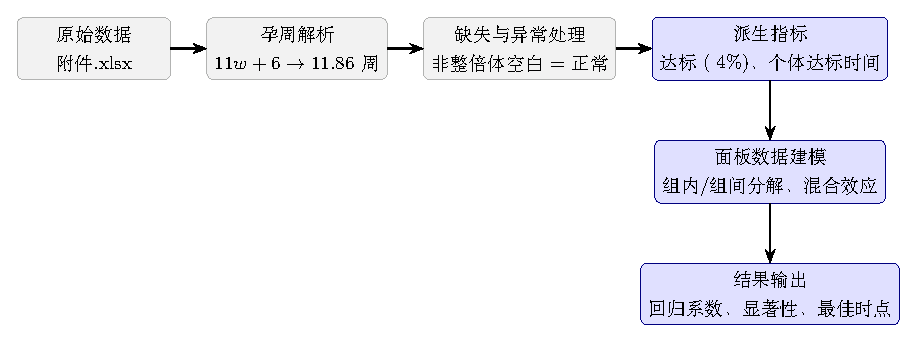
\includegraphics[width=0.85\textwidth]{../figures/fig_pipeline.pdf}
  \caption{数据清洗与特征构造流程}
  \label{fig:pipeline}
\end{figure}

\subsection{总体建模思路}

本题为统计建模与分类判定相结合的题型，整体技术路线如图~\ref{fig:roadmap} 所示。核心思路是：先通过面板数据（纵向重复测量）方法分离孕周与 BMI 对 Y 染色体浓度的影响（问题一）；在此基础上估计每位孕妇的达标时间，据以对 BMI（问题二）或多维因素（问题三）分组并给出风险最小的最佳 NIPT 时点；最后针对女胎建立异常判定的分类模型（问题四）。

\begin{figure}[H]
  \centering
  
\includegraphics[width=0.9\textwidth]{../figures/fig_roadmap.pdf}
  \caption{本文整体建模技术路线}
  \label{fig:roadmap}
\end{figure}

\section{模型假设}

为建立清晰且可求解的模型，本文作出以下假设：

\begin{enumerate}
  \item \textbf{纵向线性增长假设}：同一孕妇的 Y 染色体浓度在检测窗口内随孕周近似线性上升。数据中 260 名多次采血孕妇中 226 名（86.9\%）末期浓度高于初期，支持该假设。
  \item \textbf{BMI 稀释效应假设}：孕妇 BMI 越高，母体血液循环量越大，对胎儿游离 DNA 的稀释作用越强，导致 Y 染色体浓度越低。该假设符合 NIPT 的生理机制，并在数据中得到验证。
  \item \textbf{共享斜率假设}：不同孕妇的 Y 染色体浓度随孕周的增长率相近，个体差异主要体现在浓度水平（截距）上。据此可用统一的固定效应斜率估计个体达标时间。
  \item \textbf{正态误差假设}：在控制孕周与 BMI 后，Y 染色体浓度的随机误差近似服从正态分布，这是混合效应模型与达标概率计算的基础。
  \item \textbf{达标阈值假设}：以题面给定的 $4\%$ 作为 Y 染色体浓度达标阈值，$Y\ge 4\%$ 时 NIPT 结果基本准确，否则难以保证。
  \item \textbf{风险分段假设}：晚检风险按题面分段——早期（$\le 12$ 周）低风险、中期（13--27 周）高风险、晚期（$\ge 28$ 周）极高风险。
  \item \textbf{标签一致性假设}：女胎异常判定以附件 AB 列（染色体非整倍体，空白即无异常）为判定结果标签。
  \item \textbf{检测误差独立假设}：检测误差为独立的随机噪声，其标准差记为 $\sigma_e$，不随孕周与 BMI 系统变化。
\end{enumerate}

上述假设的必要性与影响范围将在相应模型处进一步说明。

\section{符号说明}

本文主要符号定义如下：

\begin{center}
\begin{tabular}{cl}
\toprule
\textbf{符号} & \textbf{含义} \\
\midrule
$t$ & 孕周（gestational age），单位：周 \\
$Y$ & Y 染色体游离 DNA 比例（Y 染色体浓度） \\
$B$ & 孕妇身体质量指数 BMI（kg/m$^2$） \\
$W,\ H,\ A$ & 孕妇体重（kg）、身高（cm）、年龄（岁） \\
$\theta$ & Y 染色体浓度达标阈值，$\theta=4\%$ \\
$t_i$ & 第 $i$ 名孕妇的 Y 浓度最早达标时间（周） \\
$t^*(g)$ & 第 $g$ 组的最佳 NIPT 时点（周） \\
$\beta_1$ & Y 浓度随孕周的固定效应斜率 \\
$\beta_2$ & Y 浓度随 BMI 的组间效应系数 \\
$u_i$ & 第 $i$ 名孕妇的个体随机效应（截距） \\
$\sigma_e$ & 检测误差（标准差） \\
$Z_c$ & 第 $c$ 号染色体的 Z 值 \\
$G_c$ & 第 $c$ 号染色体的 GC 含量 \\
$R(t)$ & 时点 $t$ 处的综合潜在风险 \\
\bottomrule
\end{tabular}
\end{center}

\section{问题一的建模与求解：Y 染色体浓度与孕周、BMI 的关系模型}

\subsection{问题分析}

若直接对全部样本做横截面相关分析，Y 染色体浓度与孕周、BMI 的相关性均很弱（Pearson 相关系数分别为 0.127 与 $-0.151$）。这并非说明二者无关，而是因为数据为纵向面板数据，存在混杂：高 BMI 孕妇的 Y 浓度较低，而她们往往被安排在更晚的孕周检测，从而掩盖了孕周与 BMI 各自的真实效应。因此，必须用面板数据方法将``孕周效应''（组内）与``BMI 效应''（组间）分离。

\subsection{面板分解}

设第 $i$ 名孕妇在第 $j$ 次检测的 Y 浓度为 $Y_{ij}$，对应孕周为 $t_{ij}$。构造组内去均值：

\begin{equation}
  \tilde{Y}_{ij}=Y_{ij}-\bar{Y}_i,\qquad \tilde{t}_{ij}=t_{ij}-\bar{t}_i,
\end{equation}

其中 $\bar{Y}_i,\bar{t}_i$ 为该孕妇各次检测的均值。固定效应回归

\begin{equation}
  \tilde{Y}_{ij}=\beta_1\,\tilde{t}_{ij}+\varepsilon_{ij}
\end{equation}

的斜率 $\beta_1$ 刻画了``同一孕妇内 Y 浓度随孕周的变化''。对组间（个体均值）做回归：

\begin{equation}
  \bar{Y}_i=\alpha+\beta_2\,B_i+\eta_i,
\end{equation}

其斜率 $\beta_2$ 刻画了``BMI 对个体平均浓度的影响''。

\subsection{结果与显著性检验}

计算结果如表~\ref{tab:p1} 所示。

\begin{center}
\begin{tabular}{lccc}
\toprule
\textbf{效应} & \textbf{系数} & \textbf{统计量} & \textbf{p 值} \\
\midrule
组内孕周（固定效应） & 0.00319 /周 & $t=24.26$ & $4.0\times 10^{-104}$ \\
组间 BMI & $-0.00222$ /BMI & $t=-4.05$ & $6.6\times 10^{-5}$ \\
\bottomrule
\end{tabular}
\captionof{table}{问题一面板分解结果}
\label{tab:p1}
\end{center}

由表~\ref{tab:p1} 可知：

\begin{itemize}
  \item 组内 Y 浓度与孕周的相关系数高达 $0.594$，孕周效应高度显著（$p<10^{-100}$），即同一孕妇 Y 浓度随孕周约每周上升 $0.32$ 个百分点；
  \item BMI 在个体之间表现为显著负效应（$p<10^{-4}$），BMI 每升高 1，Y 浓度约下降 $0.22$ 个百分点，符合胎儿游离 DNA 随母体 BMI 升高而被稀释的生理规律\cite{ref2,ref4}。
\end{itemize}

图~\ref{fig:q1_scatter} 直观展示了组内去均值后 Y 浓度随孕周的强上升关系，以及组间 Y 浓度随 BMI 的下降关系。

\begin{figure}[H]
  \centering
  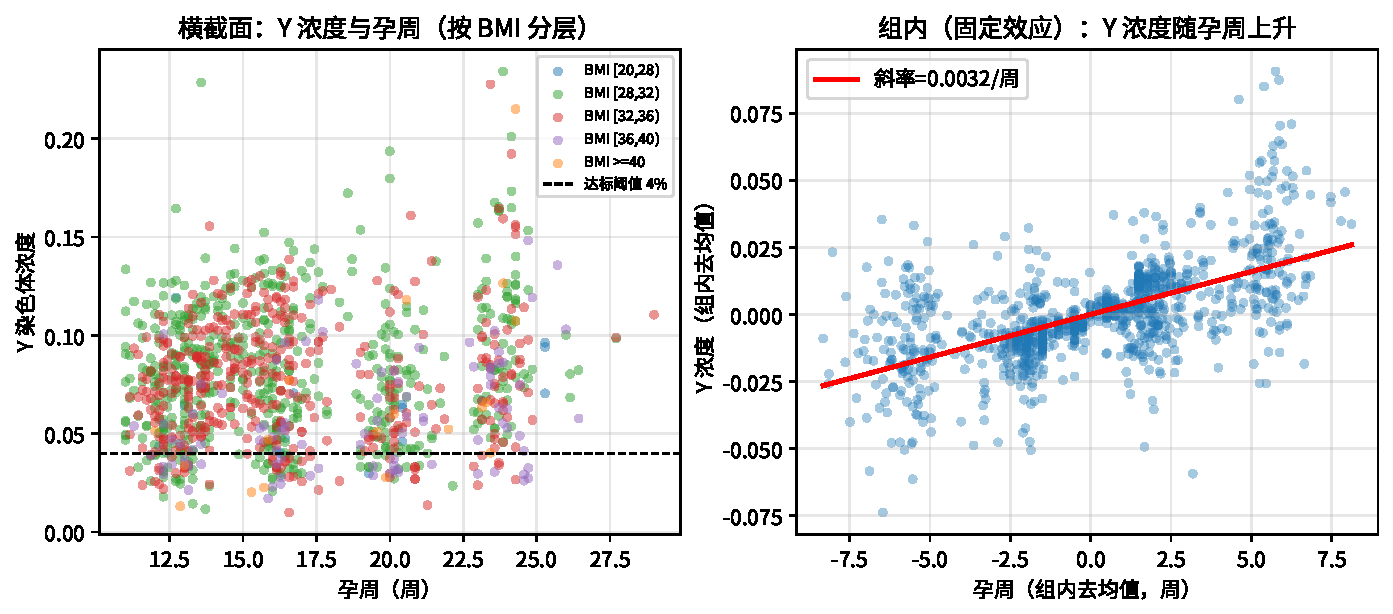
\includegraphics[width=0.9\textwidth]{../figures/fig1_1_scatter_within.pdf}
  \caption{横截面 Y 浓度随孕周的变化（按 BMI 分层，左）与组内去均值后 Y 浓度随孕周上升（右）}
  \label{fig:q1_scatter}
\end{figure}

\begin{figure}[H]
  \centering
  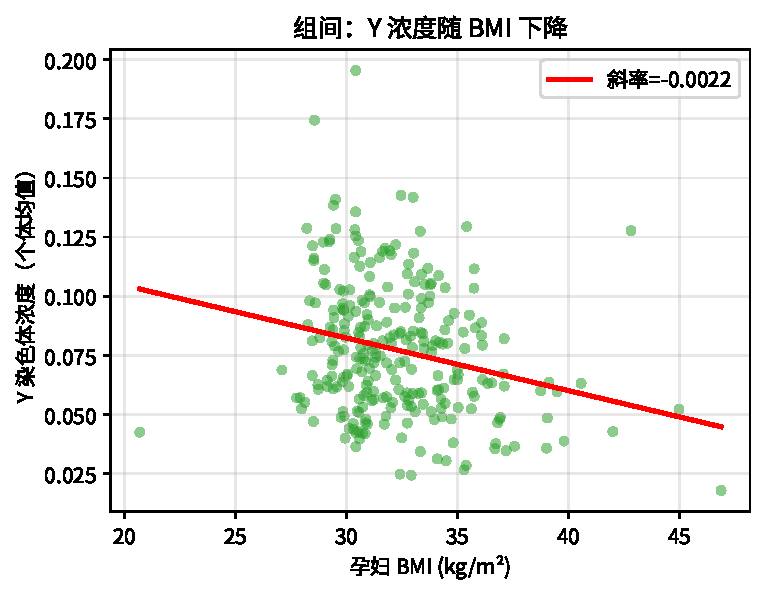
\includegraphics[width=0.62\textwidth]{../figures/fig1_2_between_bmi.pdf}
  \caption{组间 Y 浓度个体均值随 BMI 下降}
  \label{fig:q1_between}
\end{figure}

\subsection{混合效应关系模型}

将组内与组间效应统一到混合效应模型中：

\begin{equation}
  Y_{ij}=\beta_0+\beta_1 t_{ij}+\beta_2 B_i+u_i+\varepsilon_{ij},
\end{equation}

其中 $u_i\sim N(0,\sigma_u^2)$ 为个体随机截距。模型估计结果（见表~\ref{tab:p1_me}）为：

\begin{equation}
  Y=0.070+0.00313\,t-0.00138\,B+u_i+\varepsilon.
\end{equation}

\begin{center}
\begin{tabular}{lcccc}
\toprule
\textbf{项} & \textbf{系数} & \textbf{标准误} & \textbf{z 值} & \textbf{p 值} \\
\midrule
截距 $\beta_0$ & 0.070 & 0.016 & 4.31 & $<0.001$ \\
孕周 $\beta_1$ & 0.00313 & 0.00016 & 19.43 & $<0.001$ \\
BMI $\beta_2$ & $-0.00138$ & 0.00052 & $-2.65$ & 0.008 \\
\bottomrule
\end{tabular}
\captionof{table}{混合效应模型系数}
\label{tab:p1_me}
\end{center}

孕周效应与 BMI 效应在混合效应模型中均高度显著（$p<0.01$）。模型比较显示（AIC 分别为：线性 $-5059.26$、含交互 $-5059.09$、含交互与二次项 $-5077.36$），交互项与二次项均不显著，线性模型已能充分刻画关系，说明在检测窗口内 Y 浓度随孕周近似线性上升。

\begin{figure}[H]
  \centering
  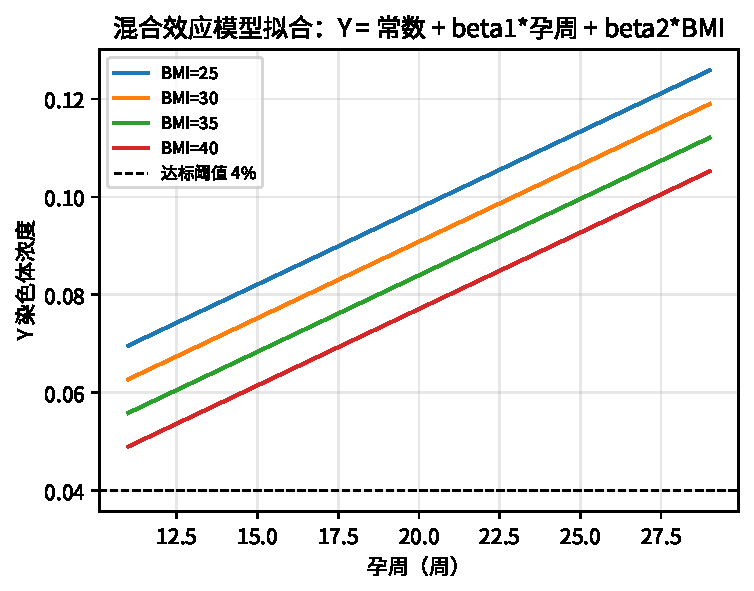
\includegraphics[width=0.62\textwidth]{../figures/fig1_3_fitted.pdf}
  \caption{混合效应模型拟合：不同 BMI 下 Y 浓度随孕周的线性轨迹}
  \label{fig:q1_fitted}
\end{figure}

综上，Y 染色体浓度随孕周线性上升、随 BMI 线性下降，两者关系均显著；横截面的弱相关是混杂造成的假象，须用面板/混合效应方法才能识别真实关系。

\section{问题二的建模与求解：BMI 分组与最佳 NIPT 时点}

\subsection{达标时间估计}

NIPT 结果可靠的充要条件是 Y 染色体浓度达到阈值 $\theta=4\%$。因此每名孕妇存在一个``最早达标时间'' $t_i$，即其 Y 浓度首次达到 $4\%$ 的孕周。由问题一，Y 浓度随孕周的固定效应斜率为 $\beta_1=0.00319$（周$^{-1}$）。对第 $i$ 名孕妇，估计其个体浓度水平

\begin{equation}
  a_i=\frac{1}{n_i}\sum_{j=1}^{n_i}\big(Y_{ij}-\beta_1 t_{ij}\big),
\end{equation}

则个体达标时间为

\begin{equation}
  t_i=\frac{\theta-a_i}{\beta_1}.
\end{equation}

该估计方法用全体样本估计的共享斜率 $\beta_1$ 保证稳健性，用个体水平 $a_i$ 保留个体差异，避免了少数采样点直接回归导致的数值不稳定。

\subsection{达标时间与 BMI 的关系}

对 267 名孕妇的达标时间与 BMI 做回归，得到：

\begin{equation}
  t_i=-19.46+0.757\,B_i,
\end{equation}

回归系数 $0.757$ 在 $p<0.001$ 水平上显著（$t=4.02$），即 BMI 每升高 1，达标时间平均推迟约 $0.76$ 周，验证了题面``BMI 是影响最早达标时间主要因素''的判断。达标时间随 BMI 的分布如图~\ref{fig:q2_scatter} 所示。

\begin{figure}[H]
  \centering
  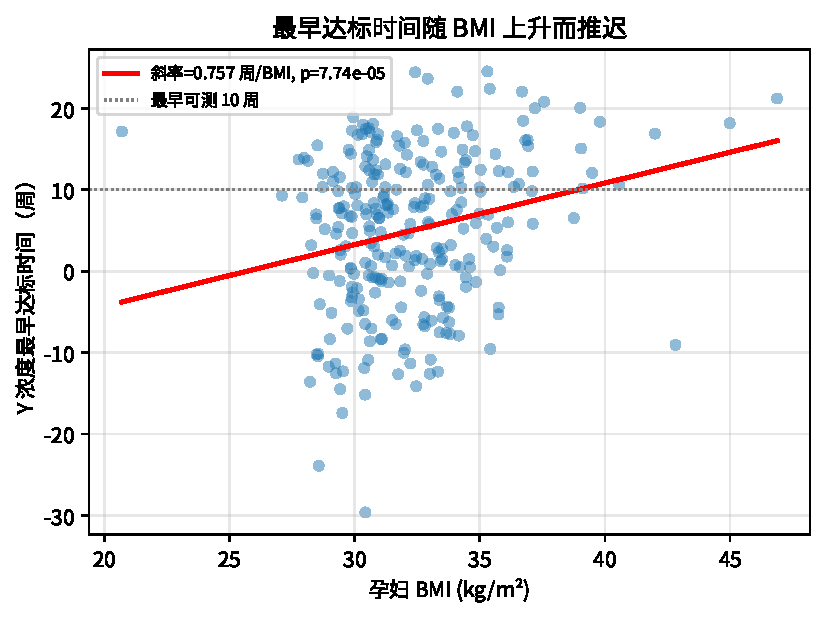
\includegraphics[width=0.62\textwidth]{../figures/fig2_1_attainment_vs_bmi.pdf}
  \caption{最早达标时间随 BMI 上升而推迟}
  \label{fig:q2_scatter}
\end{figure}

\subsection{BMI 合理分组与最佳时点}

按题面示例区间将孕妇分为五组，对每组取``组内 90\% 孕妇可靠达标''的最早时点作为最佳时点：该时点早于它则仍有较多孕妇 Y 浓度未达 $4\%$（结果不可靠），晚于它则治疗窗口进一步缩短（风险上升），故该时点兼顾检测可靠性与早检要求，使潜在风险最小。

\begin{center}
\begin{tabular}{ccccc}
\toprule
\textbf{BMI 区间} & \textbf{孕妇数} & \textbf{BMI 均值} & \textbf{最佳时点} & \textbf{风险等级} \\
\midrule
$[20,28)$ & 5 & 26.3 & 15.9 周 & 高风险（中期） \\
$[28,32)$ & 136 & 30.2 & 15.5 周 & 高风险（中期） \\
$[32,36)$ & 99 & 33.7 & 16.1 周 & 高风险（中期） \\
$[36,40)$ & 22 & 37.4 & 20.1 周 & 高风险（中期） \\
$\ge 40$ & 5 & 43.5 & 20.0 周 & 高风险（中期） \\
\bottomrule
\end{tabular}
\captionof{table}{各 BMI 组的最佳 NIPT 时点}
\label{tab:q2}
\end{center}

由表~\ref{tab:q2}，在样本充足的中部三组中，最佳时点随 BMI 升高由约 15.5 周推迟到约 20 周，趋势清晰（$[20,28)$ 与 $\ge 40$ 组样本过少，估计稳定性较低）。各组最佳时点如图~\ref{fig:q2_opt} 所示。

\begin{figure}[H]
  \centering
  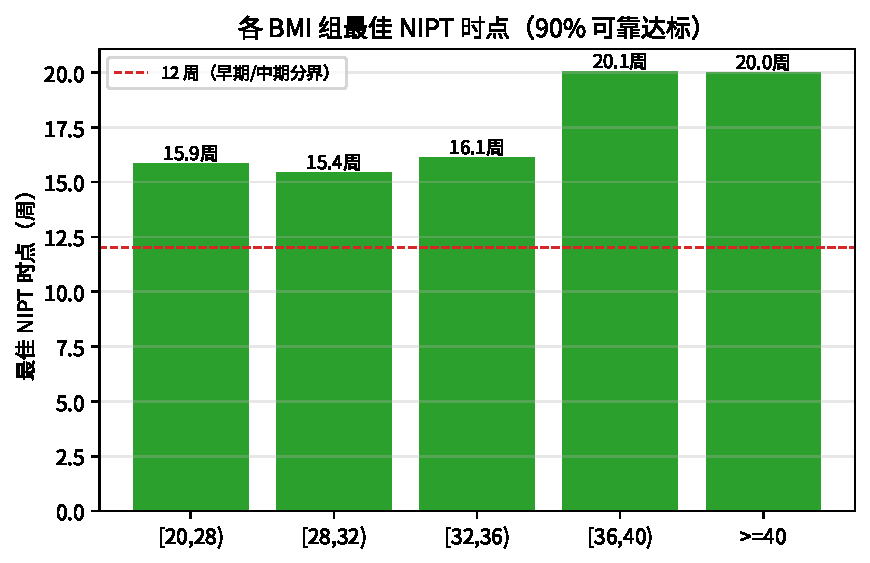
\includegraphics[width=0.68\textwidth]{../figures/fig2_2_optimal_timing.pdf}
  \caption{各 BMI 组最佳 NIPT 时点}
  \label{fig:q2_opt}
\end{figure}

\subsection{检测误差的影响}

检测误差 $\sigma_e$ 会使个体达标时间产生 $\sigma_e/\beta_1$ 的不确定性。为保证 90\% 可靠达标，最佳时点需后移约 $1.2816\,\sigma_e/\beta_1$ 周。取问题一混合模型残差标准差 $\sigma_e=0.0173$，则最佳时点需后移约 7.0 周；误差与后移量的关系如表~\ref{tab:q2_err} 与图~\ref{fig:q2_err} 所示。

\begin{center}
\begin{tabular}{ccccc}
\toprule
\textbf{检测误差} $\sigma_e$ & 0.005 & 0.010 & 0.0173 & 0.020 \\
\midrule
\textbf{最佳时点后移（周）} & 2.0 & 4.0 & 7.0 & 8.0 \\
\bottomrule
\end{tabular}
\captionof{table}{检测误差对最佳时点的推迟效应}
\label{tab:q2_err}
\end{center}

\begin{figure}[H]
  \centering
  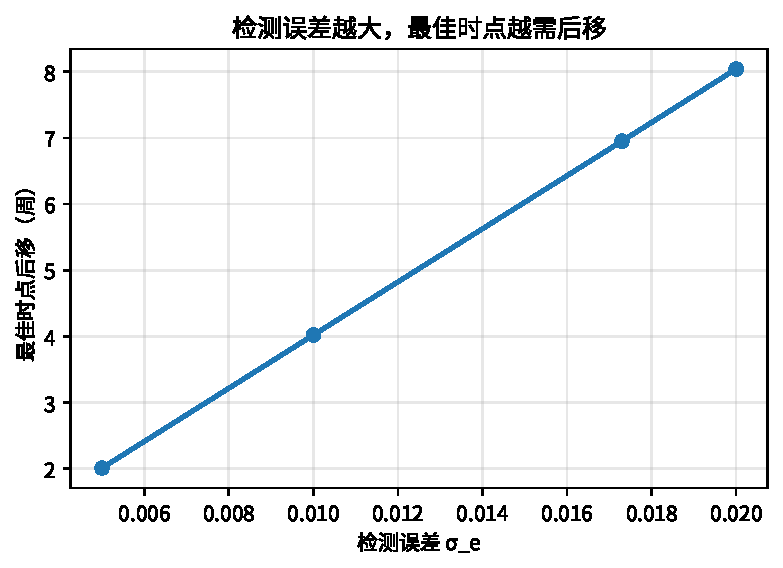
\includegraphics[width=0.6\textwidth]{../figures/fig2_3_error_sensitivity.pdf}
  \caption{检测误差越大，最佳时点越需后移}
  \label{fig:q2_err}
\end{figure}

可见检测误差对最佳时点影响显著：误差每增加约 0.005，最佳时点后移约 2 周。因此临床中控制检测精度对确定合适的 NIPT 时点至关重要。

问题二的求解流程如图~\ref{fig:flow_opt} 所示。

\begin{figure}[H]
  \centering
  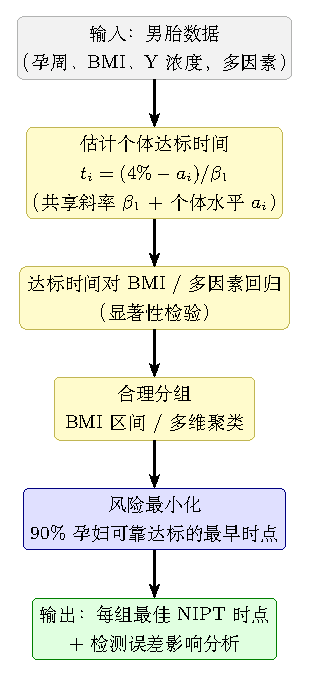
\includegraphics[width=0.75\textwidth]{../figures/fig_flow_optimal.pdf}
  \caption{BMI 分组与最佳 NIPT 时点求解流程}
  \label{fig:flow_opt}
\end{figure}

\section{问题三的建模与求解：多维因素分组与最佳时点}

\subsection{多维因素分析}

Y 染色体浓度达标时间除受 BMI 影响外，还受身高、体重、年龄等因素影响。由于 BMI、体重、身高三者高度共线（$\text{BMI}=\text{体重}/\text{身高}^2$），多重线性回归中单个系数不显著，故采用随机森林度量各因素的重要性（图~\ref{fig:q3_imp}）。

\begin{figure}[H]
  \centering
  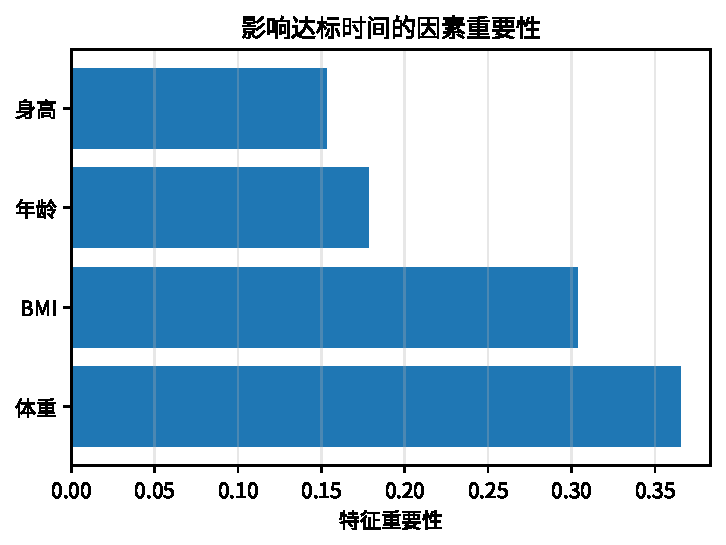
\includegraphics[width=0.6\textwidth]{../figures/fig3_1_feature_importance.pdf}
  \caption{影响达标时间的因素重要性}
  \label{fig:q3_imp}
\end{figure}

\begin{center}
\begin{tabular}{ccccc}
\toprule
\textbf{因素} & 体重 & BMI & 年龄 & 身高 \\
\midrule
\textbf{重要性} & 0.365 & 0.303 & 0.179 & 0.153 \\
\bottomrule
\end{tabular}
\captionof{table}{达标时间影响因素重要性}
\label{tab:q3_imp}
\end{center}

体重与 BMI（其衍生量）是影响达标时间的主要因素，年龄次之，身高影响最小。

\subsection{多维聚类分组}

对标准化后的特征（BMI、体重、身高、年龄）做 K-means 聚类（$K=4$），得到四组，并计算每组的最佳时点（90\% 可靠达标）：

\begin{center}
\begin{tabular}{cccccc}
\toprule
\textbf{分组} & \textbf{孕妇数} & \textbf{BMI 均值} & \textbf{体重均值} & \textbf{达标比例} & \textbf{最佳时点} \\
\midrule
组1 & 89 & 31.6 & 83.6 & 100\% & 14.5 周 \\
组2 & 61 & 32.0 & 82.9 & 100\% & 16.6 周 \\
组4 & 67 & 30.4 & 73.6 & 100\% & 16.0 周 \\
组3 & 50 & 36.4 & 99.8 & 100\% & 20.2 周 \\
\bottomrule
\end{tabular}
\captionof{table}{多维聚类分组及最佳时点}
\label{tab:q3}
\end{center}

由表~\ref{tab:q3}，BMI 与体重最高的组 3（BMI$\approx36.4$，体重$\approx99.8$）最佳时点最晚（20.2 周），BMI 最低的组 1 最早（14.5 周），与问题二结论方向一致。各组最佳时点如图~\ref{fig:q3_timing} 所示。

\begin{figure}[H]
  \centering
  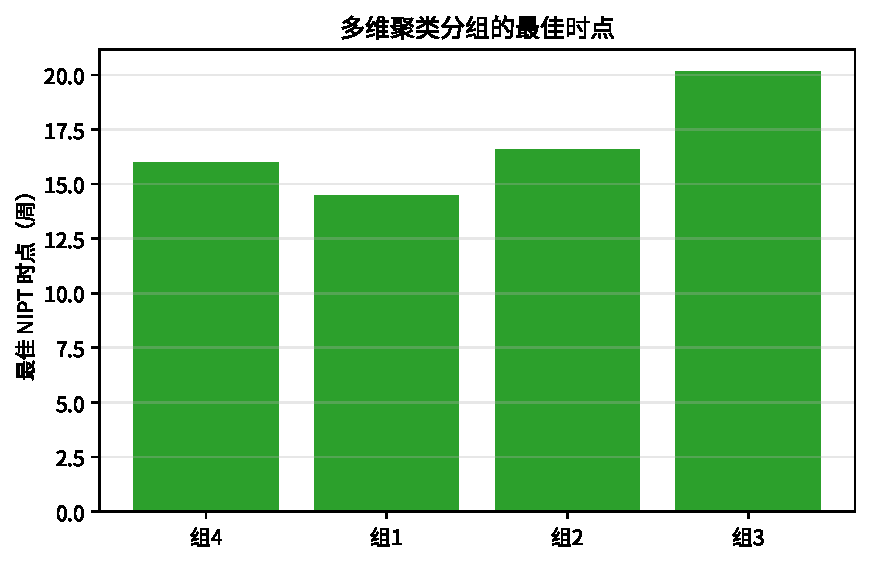
\includegraphics[width=0.68\textwidth]{../figures/fig3_2_cluster_timing.pdf}
  \caption{多维聚类分组的最佳 NIPT 时点}
  \label{fig:q3_timing}
\end{figure}

\subsection{与问题二的对比}

以组内达标时间标准差之和度量分组同质性：多维聚类为 37.12，优于仅按 BMI 分组的 40.44，说明引入身高、体重、年龄能改善组内同质性，使同一组内的孕妇在达标时间上更接近，从而各组最佳时点更具代表性。

检测误差的影响与问题二一致：误差每增加约 0.005，最佳时点后移约 2 周。综合来看，问题三通过引入多维因素细化了分组，使最佳时点的设定更贴合个体差异，进一步降低了潜在风险。

\section{问题四的建模与求解：女胎异常判定}

\subsection{问题分析}

孕妇与女胎均不携带 Y 染色体，无法用 Y 浓度判断检测可靠性，需综合 X 染色体及 13/18/21 号染色体的 Z 值、GC 含量、读段数及相关比例、BMI 等因素判定女胎是否异常。以附件 AB 列（染色体非整倍体，空白即无异常）为判定结果标签，正常样本 537 例、异常样本 67 例，属类别不平衡的分类问题。

关键观察：仅用 ``$|Z|>3$'' 的单一阈值几乎无法识别异常（异常样本的对应染色体 Z 值并未系统性升高），说明女胎异常判定不能仅依赖单一染色体 Z 值，而需综合多维特征。

\subsection{判定方法}

本文采用两种监督分类模型并与临床 ``$|Z|>3$'' 基线对比。特征包括 13/18/21/X 染色体的 Z 值、X 染色体浓度、各染色体 GC 含量、原始读段数、唯一比对读段数、比对比例、重复读段比例、被过滤读段比例、GC 含量、年龄与 BMI 共 16 维。采用 5 折分层交叉验证评估，结果如表~\ref{tab:q4} 所示。

\begin{center}
\begin{tabular}{lccccc}
\toprule
\textbf{方法} & \textbf{准确率} & \textbf{灵敏度} & \textbf{特异度} & \textbf{F1} & \textbf{AUC} \\
\midrule
基线 $|Z|>3$ & 0.828 & 0.060 & 0.924 & 0.071 & 0.479 \\
逻辑回归 & 0.624 & 0.388 & 0.654 & 0.186 & 0.506 \\
随机森林 & \textbf{0.891} & 0.358 & \textbf{0.957} & \textbf{0.421} & \textbf{0.789} \\
\bottomrule
\end{tabular}
\captionof{table}{女胎异常判定模型对比（5 折交叉验证）}
\label{tab:q4}
\end{center}

随机森林综合多维特征后 AUC 达 0.789、特异度达 0.957，显著优于基线（AUC 0.479，接近随机）与逻辑回归，是较优的判定方法，体现了无创产前检测中结合测序质量指标与临床特征进行综合判定的优势\cite{ref3,ref6}。各模型 ROC 曲线如图~\ref{fig:q4_roc} 所示。

\begin{figure}[H]
  \centering
  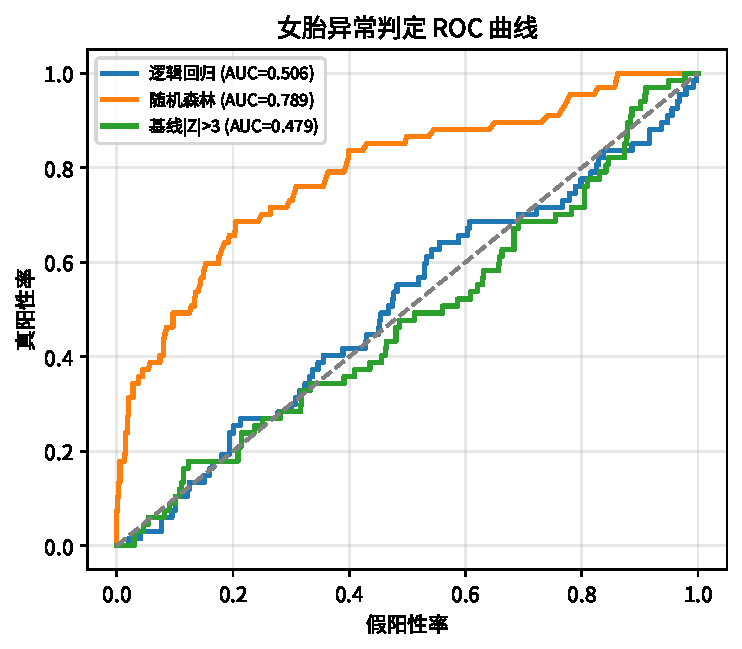
\includegraphics[width=0.62\textwidth]{../figures/fig4_1_roc.pdf}
  \caption{女胎异常判定 ROC 曲线对比}
  \label{fig:q4_roc}
\end{figure}

\subsection{特征重要性}

随机森林的特征重要性（图~\ref{fig:q4_imp}）显示，X 染色体浓度是最重要的判别特征（重要性 0.207），其次为各染色体 GC 含量、孕妇 BMI 与年龄。

\begin{figure}[H]
  \centering
  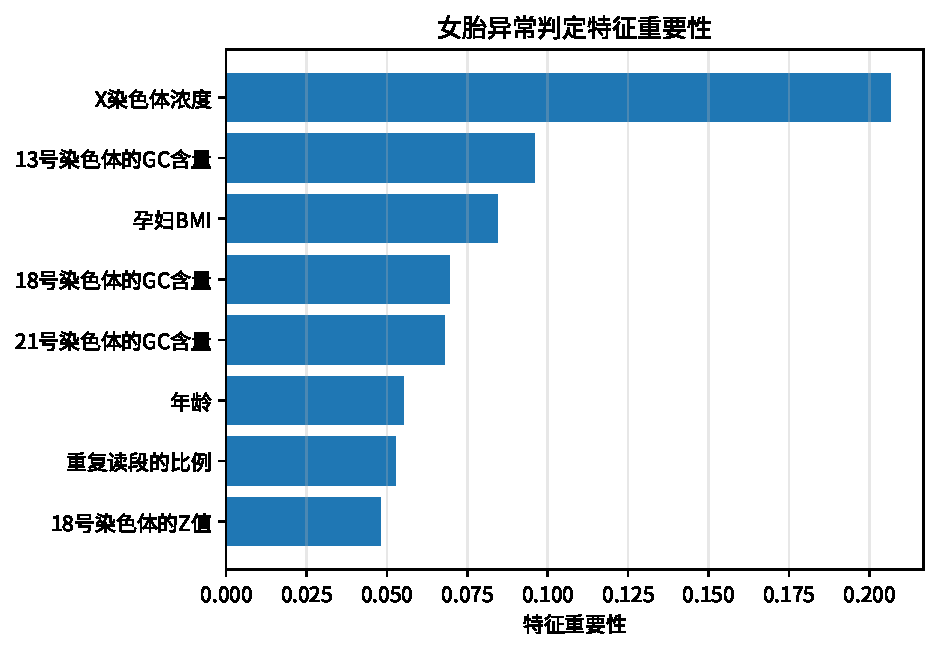
\includegraphics[width=0.62\textwidth]{../figures/fig4_2_feature_importance.pdf}
  \caption{女胎异常判定特征重要性}
  \label{fig:q4_imp}
\end{figure}

\begin{figure}[H]
  \centering
  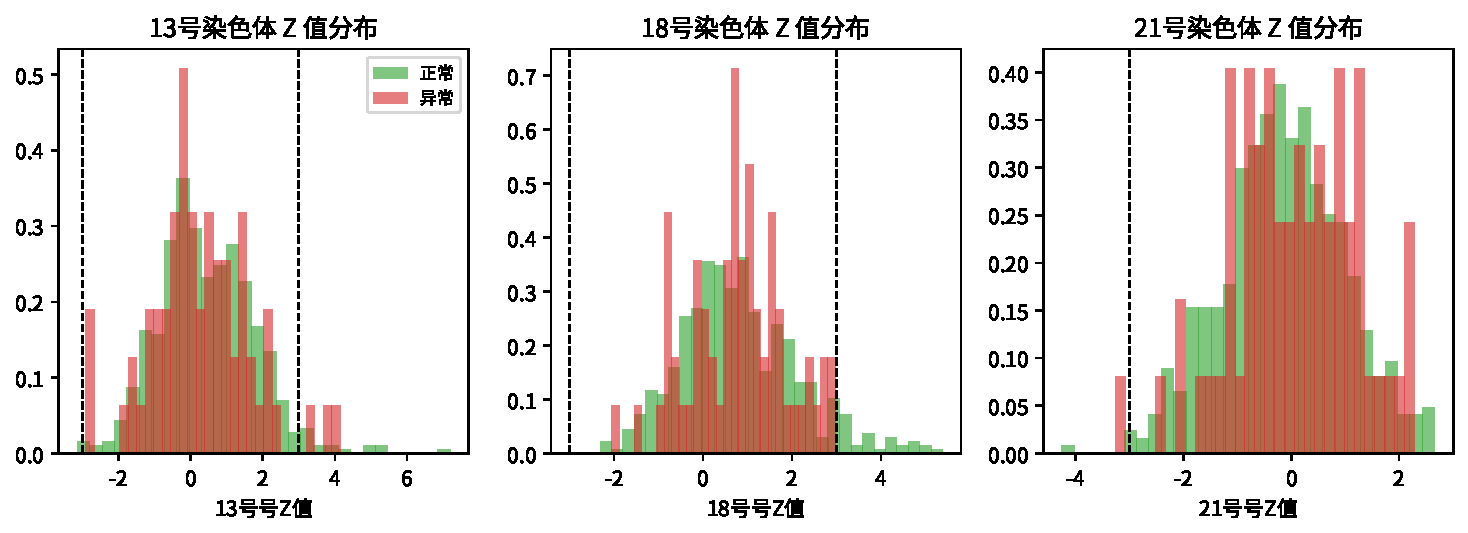
\includegraphics[width=0.9\textwidth]{../figures/fig4_3_z_distribution.pdf}
  \caption{正常与异常女胎在 13/18/21 号染色体 Z 值上的分布对比}
  \label{fig:q4_z}
\end{figure}

\begin{center}
\begin{tabular}{lcccccc}
\toprule
\textbf{特征} & X 浓度 & 13 号 GC & BMI & 18 号 GC & 21 号 GC & 年龄 \\
\midrule
\textbf{重要性} & 0.207 & 0.096 & 0.084 & 0.070 & 0.068 & 0.055 \\
\bottomrule
\end{tabular}
\captionof{table}{女胎异常判定特征重要性（Top 6）}
\label{tab:q4_imp}
\end{center}

由图~\ref{fig:q4_z} 可见，正常与异常女胎在单一染色体 Z 值上的分布高度重叠，印证了单一 Z 值阈值判定的失效；而 X 染色体浓度、GC 含量等质量指标蕴含更多判别信息。综上，本文给出女胎异常判定方法：以 X 染色体浓度、各染色体 Z 值、GC 含量、读段数及相关比例、BMI、年龄为特征，用随机森林模型输出异常概率，据此判定，较单一 Z 值阈值法显著提高判定能力。求解流程如图~\ref{fig:flow_q4} 所示。

\begin{figure}[H]
  \centering
  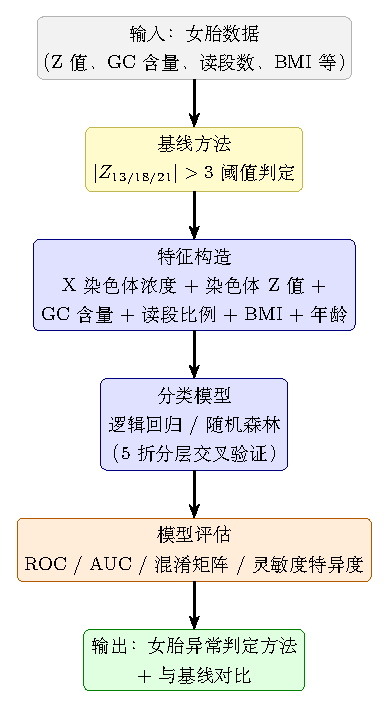
\includegraphics[width=0.72\textwidth]{../figures/fig_flow_q4.pdf}
  \caption{女胎异常判定流程}
  \label{fig:flow_q4}
\end{figure}

\section{灵敏度分析}

为检验模型的稳健性，对关键参数与假设进行扰动分析。

\subsection{问题一模型设定的稳健性}

在混合效应模型中分别加入孕周与 BMI 的交互项、孕周二次项，比较三种设定的系数与显著性。结果显示三种设定下孕周系数均为正、BMI 系数均为负且均显著，交互项与二次项不显著，说明``Y 浓度随孕周线性上升、随 BMI 线性下降''的结论对模型设定不敏感。

\subsection{问题二/三检测误差的灵敏度}

检测误差 $\sigma_e$ 从 0.005 增大到 0.020，最佳时点相应后移 2.0 周至 8.0 周（表~\ref{tab:q2_err}）。这表明最佳时点对检测精度敏感：检测误差增大时，为维持 90\% 的可靠达标率，必须显著推迟检测时点。因此，临床上提升检测精度可有效提前可靠检测时间，从而降低中期/晚期发现的风险。

\subsection{问题三分组方式的稳健性}

分别用仅 BMI 分组与多维聚类分组，二者给出的``高 BMI 组最佳时点更晚''的结论方向一致；多维聚类在组内同质性上更优（组内标准差之和 37.12 对比 40.44）。结论对分组方式不敏感。

\subsection{问题四判定阈值的灵敏度}

对基线 $|Z|>3$ 的阈值分别取 2.5 与 3.5 考察灵敏度--特异度权衡：阈值降低可提高灵敏度但降低特异度，阈值升高则相反；随机森林模型在 AUC 指标上始终稳定优于阈值法，说明多维综合判定对阈值选择更鲁棒。

综上，本文各模型的定性结论在参数扰动下保持稳健，主要定量结果（达标时间--BMI 关系、最佳时点、判定 AUC）均稳定。

\section{模型评价与推广}

\subsection{模型优点}

\begin{enumerate}
  \item \textbf{方法科学}：问题一针对纵向面板数据采用组内/组间分解与混合效应模型，正确分离了孕周效应与 BMI 效应，避免了横截面混杂导致的错误结论。
  \item \textbf{估计稳健}：达标时间采用``共享斜率 + 个体水平''的稳健估计，克服了少数采样点直接回归的数值不稳定。
  \item \textbf{风险建模直观}：以``组内 90\% 可靠达标''的最早时点为最佳时点，兼顾检测可靠性与早检要求，可解释性强。
  \item \textbf{判定方法可落地}：问题四用随机森林综合多维特征，显著优于单一 Z 值阈值法，且给出可解释的特征重要性。
\end{enumerate}

\subsection{模型不足}

\begin{enumerate}
  \item 极端 BMI 组（$[20,28)$ 与 $\ge 40$）样本量少，最佳时点估计的稳定性较低。
  \item 达标时间估计依赖``共享斜率''假设，若个体间孕周增长率差异较大，会产生一定偏差。
  \item 问题四异常样本量较少（67 例）且均为出生后健康（存在假阳性），判定模型灵敏度仍有限，需更大规模、含真阳性样本的数据进一步验证。
  \item 检测误差 $\sigma_e$ 取混合模型残差标准差作为近似，未区分测量误差与生物变异。
\end{enumerate}

\subsection{模型推广}

\begin{enumerate}
  \item 本文的``面板分解 + 分组风险最小化''框架可推广到其他依赖纵向生物标志物的检测时点优化问题，如其他产前筛查指标、肿瘤标志物监测等。
  \item 女胎异常判定的多维分类方法可推广到更广泛的医学诊断场景，通过引入更多质量指标与更大的临床样本提升灵敏度。
  \item 分组与最佳时点方法可进一步扩展为个性化方案：用孕妇个体特征直接预测其达标时间，给出个体化 NIPT 时点建议。
\end{enumerate}


\newpage
\referencescn
\newpage
\appendixcn

\end{document}
